\documentclass{chi-ext}
\copyrightinfo{ }

\title{Duo-Portal, a HTML5 cooperative game}

\numberofauthors{2}
\author{
  \alignauthor{
  	\textbf{Frederico Schardong}\\
  	\affaddr{University of Calgary}\\
  	\affaddr{Calgary, CA T2N 1N4 Canada}\\
  	\email{fschardo@ucalgary.ca}
  }\alignauthor{
  	\textbf{Cedricson Chapeu}\\
  	\affaddr{University of Calgary}\\
  	\affaddr{Calgary, CA T2N 1N4 Canada}\\
  	\email{cedricson@ucalgary.ca}
  }
}

% Paper metadata (use plain text, for PDF inclusion and later re-using, if desired)
\def\plaintitle{Duo-Portal, a HTML5 cooperative game}
\def\plainauthor{Frederico Schardong}
\def\plainkeywords{Cooperative, HTML5, online game, portal}
\def\plaingeneralterms{Cooperative, HTML5, online game, portal}

\hypersetup{
  % Your metadata go here
  pdftitle={\plaintitle},
  pdfauthor={\plainauthor},  
  pdfkeywords={\plainkeywords},
  pdfsubject={\plaingeneralterms},
  % Quick access to color overriding:
  citecolor=black,
  linkcolor=blue,
  menucolor=black,
  urlcolor=blue,
}

\usepackage{graphicx}   % for EPS use the graphics package instead
\usepackage{balance}    % useful for balancing the last columns
\usepackage{bibspacing} % save vertical space in references

\begin{document}

\maketitle

\begin{abstract}
In this paper we describe the implementation of a cooperative online game in HTML5 inspired in the successful game Portal by Valve.
\end{abstract}

\category{H.5.m}{Information interfaces and presentation (e.g., HCI)}{Miscellaneous}. 

\terms{\plaingeneralterms}

\section{Introduction}
This format is to be used for submissions that are published in the conference extended abstracts.  
We wish to give this volume a consistent, high-quality appearance. 
We therefore ask that authors follow some simple guidelines. 
In essence, you should format your paper exactly like this document. 
The easiest way to do this is simply to download a template from the conference website and replace the content with your own material.

\begin{figure}
\hspace*{-0.4\columnwidth}% displace figure
\parbox{1.4\columnwidth}{
  \centering
  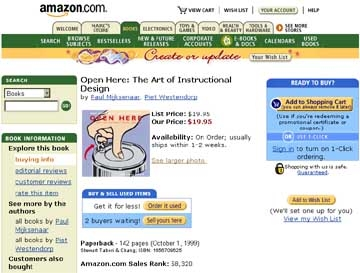
\includegraphics[width=1.4\columnwidth]{sample.jpg}
  \caption{Insert a caption below each figure. Images can "float" around body text, like this example.}
  \label{fig:sample}
}
\end{figure}

\section{Design Principles}

\section{Implementation Details}

\section{Design Evolution}

\section{Discussion and Conclusion}

\balance
\bibliographystyle{acm-sigchi}
\bibliography{sample}

\end{document}